\documentclass[a4paper]{article}
\usepackage[utf8]{inputenc}
\usepackage[catalan]{babel}
\usepackage{amsmath}
\usepackage{amsfonts}
\usepackage{amssymb}
\usepackage{graphicx}
\usepackage{float}
\author{Joan Puigcerver Pérez}
\title{Quantificació de les millores en la segmentació del cos central del text manuscrit utilitzant tècniques d'aprenentatge supervisat}
\begin{document}
\maketitle

El reconeixement de text manuscrit (HTR) és una aplicació paradigmàtica del reconeixement de formes. En particular, el reconeixement de text manuscrit \emph{offline} és una aplicació de gran interès ja que pot ser utilitzat, per exemple, per a transcriure el text de llibres i manuscrits antics per tal de preservar la informació o facilitar la cerca del seu contingut. \\

Un dels principals problemes del reconeixement de text manuscrit \emph{offline}, front a altres tasques de reconeixement, és que gran part de la variabilitat que es troba en les imatges que contenen text digitalitzat no aporta cap informació rellevant per a la classificació del text i dificulta aquesta tasca. Per exemple, un mateix autor no escriu un mateix símbol sempre de la mateixa forma, ni de la mateixa grandària i ni tan sols amb la mateixa orientació; i l'objectiu és que tots aquests diferents traços siguen classificats de la mateixa manera. Per això, un dels components fonamentals de qualsevol sistema de reconeixement de l'escriptura és la normalització d'aquesta imatge, un procés que tracta de reduir aquesta variabilitat. \\

Un pas que afecta a diferents parts de la normalització de la imatge és la segmentació del cos central del text en la imatge (veure figura \ref{fig:adlines}). Diferents sistemes utilitzen diferents tècniques per a segmentar el cos central de la línia. L'objectiu d'aquest projecte és el de comparar i quantificar les diferències entre dues d'aquestes tècniques, una basada en un enfocament heurístic \cite{Pastor07} i una altra basada en tècniques d'aprenentatge supervisat \cite{Espana10}. Les tècniques d'aprenentatge supervisat ofereixen un millor ajustament al perfil del text contingut en la imatge, però el principal inconvenient és que requereixen la intervenció d'un humà durant l'entrenament de l'eina. El resultat d'aquest projecte ajudarà a prendre la decisió d'actualitzar l'eina de detecció de línies ascendents i descendents en un sistema que actualment utilitza la tècnica heurística, proveint als responsables amb dades dels beneficis obtinguts a l'utilitzar les tècniques d'aprenentatge supervisat.

\begin{figure}[H]
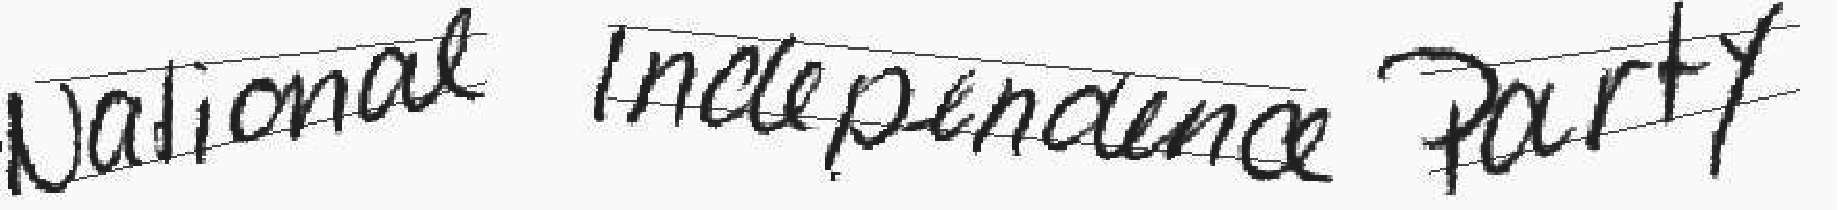
\includegraphics[width=\textwidth]{a01-011x-01_final}
\caption{Segmentació del cos central en una línia de text.}
\label{fig:adlines}
\end{figure}

\begin{thebibliography}{9}
\bibitem{Pastor07} M. Pastor. \emph{Aportaciones al Reconocimiento Automático de Texto Manuscrito}. Ph.D. Thesis. 2007.

\bibitem{Espana10} S.Espana-Boquera, M.J.Castro-Bleda, J.Gorbe-Moya,F.Zamora-Martínez. \emph{Improving Offline Handwritten Text Recognition with Hybrid HMM/ANN Models}. IEEE Transactions on Pattern Analysis and Machine Intelligence. vol. 99. 2010.
\end{thebibliography}

\end{document}